%%
%% Author: Alexander Telich
%% 2/14/18
%%

% Preamble
\documentclass[11pt]{article}
\usepackage[utf8]{inputenc}
\usepackage{amsmath}

% Packages
\usepackage{a4wide}
\usepackage{listings}
\usepackage{indentfirst}
\usepackage{graphicx}

\lstdefinestyle{mystyle}{
basicstyle=\footnotesize,
breakatwhitespace=false,
breaklines=true,
captionpos=b,
keepspaces=true,
numbers=left,
numbersep=5pt,
showspaces=false,
showstringspaces=false,
showtabs=false,
tabsize=2
}

\lstset{style=mystyle}

\author{Alexander Telich}
\title{EECS 531 A1 Exercise 1}
\date{February 19, 2018}
\graphicspath{C:/Users/ateli/Documents/School/Spring 2018/EECS 531/Assignments/531_A1/A1/Exercise1}

% Document
\begin{document}
    \maketitle
    \section{Image Blur}\label{sec:exercise1}
    \subsection{The Gaussian Kernel}\label{subsec:1. The Gaussian Kernel}
    \setlength\parindent{24pt}
    To get the desired effect of blurring an image a kernel matrix must be convoluted with
    an equal size matrix of pixel color values based on patches taken from the original image.
    The 2D Gaussian function is defined in equation (1).
    Equation (2) shows the process of convolution.
    The matrix on the left being the kernel matrix and the matrix on the right, the matrix
    you are operating on.

    \begin{equation}
        G\left(x,\ y\right)=\frac{1}{2\pi\sigma^2}e^{-\frac{x^2+y^2}{2\sigma^2}}
    \end{equation}
    {\small \begin{center}
                where $G\left(x,\ y\right)$ is the gaussian transformation at point $\left(x,\ y\right)$\\
    \end{center}}
    \newline

    \begin{equation}
        \left(\left[\begin{matrix}
                        a&b&c\\d&e&f\\g&h&i\\
        \end{matrix}\right]\ast\left[\begin{matrix}
                                         1&2&3\\4&5&6\\7&8&9\\
        \end{matrix}\right]\right)\left[center\right]=\left(i\cdot1\right)+\left(h\cdot2\right)+\left(g\cdot3\right)+\left(f\cdot4\right)+\left(e\cdot5\right)+\left(d\cdot6\right)+\left(c\cdot7\right)+\left(b\cdot8\right)+\left(a\cdot9\right)
    \end{equation}
    {\small \begin{center}
                where the left matrix is the kernel matrix, the right matrix is the
                matrix you are operating on, and [center] is the center coordinates of each
                matrix
    \end{center}}
    \section{Code}\label{sec:codeExplanation}
    \lstinputlisting[language=Python]{Exercise1.py}

    \begin{figure}[h]
        \flushleft
        \caption{Original Image}
        \centering
        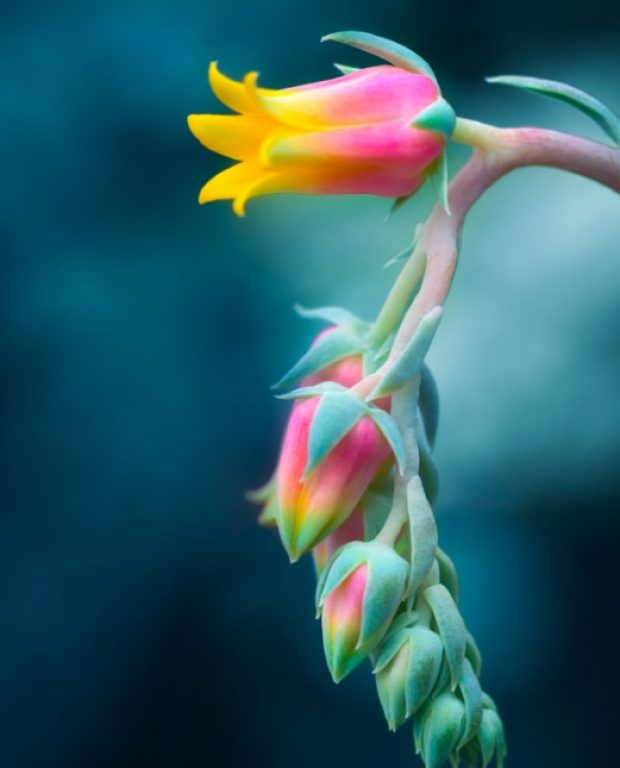
\includegraphics[scale=0.4]{Exercise1_Image.jpg}
        \caption{Image After Gaussian Blur Applied}
        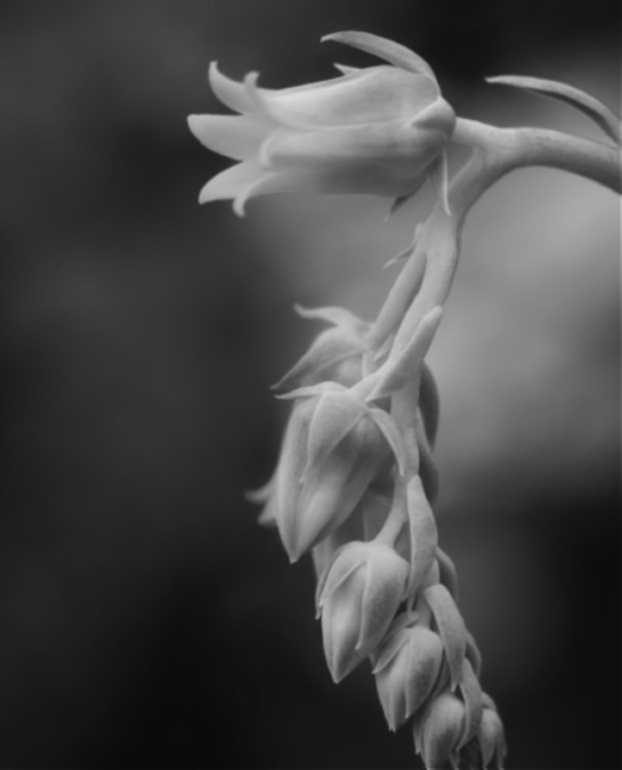
\includegraphics[scale=0.31]{Exercise1_OutputImage.png}
    \end{figure}


\end{document}
\begin{document}



\end{document}
\begin{document}



\end{document}